\documentclass[oneside,a4paper,titlepage]{article}
\usepackage{blindtext}
\usepackage[utf8]{inputenc}
\usepackage{pdfpages}
\usepackage{graphicx}
\usepackage{geometry}
\usepackage{float}
\usepackage[hidelinks]{hyperref}
\begin{document}
\begin{titlepage}
  %\toprule[2pt]
  %\midrule
  \vspace{0.2cm}
  \begin{center}
    \Huge{\textbf{P1 - Procesanalyse}}
  \end{center}
  \vspace{0.2cm}
  %\midrule
  %\toprule{2pt}
  \begin{center}
    \Large{\textbf{Gruppe B2-28}}\\
    Morten Rask Andersen\\
    Anton Christensen\\
    Lasse Fribo Gadegaard\\
    Christian Mønsted Grünberg\\
    Mathias Ibsen\\
    Mathias Rohde Pihl
  \end{center}
  \begin{center}
    22/12-2015\\
    Aalborg Universitet\\
    Software, 1. semester
  \end{center}
\end{titlepage}





\section{Indledning}

Formålet med procesanalysen er, at se tilbage på den arbejdsproces, der ligger bag udarbejdelsen af P1-projektet. Først beskrives projektets overordnede forløb samt anvendte metoder og værktøjer. Herefter vurderes hvilke dele af projektet, som gik godt, og hvilke dele der gik mindre godt. Efter vurderingen analyseres og argumenteres hvorfor de forskellige dele af projektet gik som de gjorde. Til sidst præsenteres operationelle anbefalinger til at forbedre næste projektforløb. 

\section{Beskrivelse}
\label{sec:beskrivelse}
I dette afsnit beskrives arbejdsprocessen bag de forskellige faser i projektet. Heraf beskrives de anvendte metoder og værktøjer til tidsplanlægning, opgavefordeling, samt kode- og rapportskrivning.

\subsection{Opstart}

Lige efter gruppedannelsen diskuterede vi internt i gruppen, hvilket emne indenfor projektforslaget 'Raytracing' vi ville arbejde med. Dette var en langvarig proces. Vi forsøgte først, at finde emnet vi ville arbejde med ved brug af teknikken 'brainstorm' under den kreative platform \cite{kreativ_platform}. Brainstormen kan ses i bilag \ref{sec:brainstorm} og viser gruppens første emneforslag. Formålet med den kreative platform er, at få alle vores ideer og tanker omkring projektforslaget på tavlen. Herefter forsøgte vi, vha.\ diskussion i gruppen, at udvælge de ideer vi synes passede bedst til projektforslaget. Dette var svært at vurdere, da projektforslaget ikke centrede sig om et kontekstuelt problem, men nærmere om en metode til løsning af sådan et problem. Derfor kunne vi ikke undgå at tænke løsningsorienteret. For at undgå dette måtte vi se anderledes på projektforslaget. Dette gjorde vi ved at tænke over hvad raytracing kan, i stedet for hvad det er. Det vi kom frem til var, at raytracing var en teknik til visualisering. Herefter kunne vi se på problemer, der omhandlede mangel på visualisering. Vi afgrænsede os herefter til to problemer, heraf mangel på visualisering af vindmøllers placering samt problemer med at visualisere belysningen fra lamper. Efter en diskussion i gruppen valgte vi at arbejde med det initierende problem "Kunden kan ikke visualisere, hvordan lys udbreder sig fra en lampe uden at købe og installere lampen". 

\subsection{Udarbejdelse af problemformulering}
Efter det initierende problem påbegyndte vi arbejdet med problemanalysen. I problemanalysen benyttede vi os af den kvalitative metode til, at få mere viden om det initierende problem gennem korrespondance med lampedesignere og en belysningskonsulent \cite{kvalitativ_metode}. Ud fra analysen af problemfeltet opstillede vi den endelige problemformulering. Problemformuleringen bestod af et overordnet forskningsspørgsmål og tre underspørgsmål.

\subsection{Planlægning}
I forbindelse med opstarten og udarbejdelsen af problemformuleringen, blev der udarbejdet en overordnet tidsplan til hvornår vi skulle have de store emner færdiggjort (se bilag \ref{sec:tidsplan}). Ud fra tidsplanen sørgede vi for at give os selv opgaver og deadlines løbende, så denne tidsplan blev overholdt. I starten af projektet havde vi en del hjemmeopgaver, hvor vi anvendte værktøjet 'Trello' til at overholde tidsplanen. Trello bruges til at uddele og holde styr på opgaver, og man kan på den måde danne sig et overblik over de forskellige opgaver. Et udklip af vores brug af værktøjet Trello af vist i bilag \ref{sec:trello}
\newline

\subsection{Arbejdet}
Ud fra den overordnede tidsplan blev der hver morgen lavet en dagsplan, som beskrev konkrete opgaver for hvad, der skulle nås på dagen. Et par eksempler på dagsordnen er vist herunder:

\paragraph{Dagsorden 9/10/15:}
\begin{itemize}
  \item Brainstorm.
  \item Diskussion af spørgsmål til styringsgruppemødet.
  \item Agenda.
  \item Find de programmer vi vil bruge til projektarbejde, heraf undersøg Trello, og Github.
  \item Opsummering og afrunding  af dagen.
\end{itemize}

\paragraph{Dagsorden 14/12/15:}
\begin{itemize}
  \item Revidere afgrænsning af løsningsforslag.
  \item Skrive afsnit om rotationsmatricer i udviklingsafsnittet.
  \item Fordele og ulemper ved augmented reality.
  \item Skitse til Phong.
  \item Ret sekvensdiagram.
  \item Skriv testafsnit færdigt.
\end{itemize}

Ud fra dagsorden uddelte vi arbejdsopgaver, og måden dette foregik på var, at gruppens medlemmer selv havde indflydelse på, hvilke ting, fra dagsorden, de ville skrive om. Opgaverne blev udført individuelt eller i mindre grupper. Derudover blev der ikke altid taget højde for omfanget af opgaverne, så det endte nogle gange med, at en person havde en 30 minutters opgave mens en anden person havde en to timers opgave. I slutningen af dagen eller dagen efter holdte vi korte og uformelle møder, hvor vi gennemgik og diskuterede resultaterne af opgaveskrivningen. I forbindelse med opgaveskrivningen benyttede vi os af værktøjet Git til at administrere forskellige versioner af rapporten, og på den måde sørge for, at vi alle havde tilgang til den nyeste version af rapporten. Derudover blev rapporten skrevet i 'LaTeX' som bl.a.\ gjorde det muligt at opdele rapporten i flere filer.

Med hensyn til arbejdsfordelingen har vi ikke haft en snak i gruppen om, hvad vi forventede af hinanden. Der var dog nogle forventninger, der på forhånd var aftalt som f.eks.\ at vi mødte ind til aftalt tid og, at man udførte det arbejde som blev aftalt. 

I arbejdsfasen brugte vi forskellige metoder til informationssøgning, heraf blev den usystematiske metode anvendt når der blot skulle dannes et hurtigt overblik over nye emner \cite{SO_bog}. Derudover blev der søgt information til rapporten ved brug af ekspertmetoden idet vi tog kontakt til designere og belysningskonsulenter \cite{SO_bog}. Når der var dannet overblik over det nye stof, og der skulle findes kilder der understøttede udsagn i rapporten anvendte vi den strukturerede metode, som går ud på at finde en relevant kilde, og se på hvilken anden litteratur denne kilde henviser til, og herudfra finde frem til pålidelige og gode kilder som passer præcis til de udsagn som skulle underbygges \cite{SO_bog}. 

Udover at opnå ny viden ved hjælp af ekstern informationssøgning havde forskellige gruppemedlemmer en forhåndsviden indenfor forskellige emner. Vi brugte derfor 'Peer-Learning' til at udveksle viden internt i gruppen. Dette foregik ved at personen, som havde en forhåndsviden indenfor emnet gav en præsentation på tavlen for de andre gruppemedlemmer. Dette gjorde sig også gældende i andre kurser, der foregik sideløbende med projektet.

I forbindelse med udviklingen af programmet har gruppen anvendt "Top-down programmering", som er en metode til systematisk udvikling af programmer \cite{top_down_programming}. Metoden går ud på, at opdele et overordnet problem i underproblemer, som igen kan opdeles i yderligere underproblemer.

\subsection{Afslutning}

I stedet for, at se projektet som ét stort produkt der skulle afleveres, valgte vi at inddele projektet i mindre dele, heraf problemanalysen og problemløsningen. Dette gjorde, at vi først udelukkende fokuserede på at færdiggøre problemanalysen, som efter statusseminaret blev afsluttet. Vi kunne herefter fokusere på at udarbejde og afslutte problemløsningen. 
I afslutningen af projektet rettede vi hele rapporten, og sørgede for, at der var en rød tråd igennem alle afsnit.

\subsection{Evaluering}

I slutningen af projektet blev der foretaget en gruppeevaluering. Formålet med dette var at diskutere samarbejdet i gruppen og arbejdsprocessen igennem projektet. Referatet af gruppeevalueringen kan ses i bilag \ref{sec:gruppeevaluering}.

\section{Vurdering}
Ud fra afsnit \ref{sec:beskrivelse} er der vurderet følgende:
\begin{itemize}
  \item Opgaveuddeling ved hjælp af Trello gik godt i starten og knap så godt i slutningen af projektet.
  \item Git som version-control var rigtigt god til at holde styr på koden, men knap så god til LaTeX.
  \item Dagsordenerne gik godt, men nogle gange var de meget korte og upræcise.
  \item Gennemgang af rettelser på projektet var godt.
  \item Fællesregning af gruppeopgaver fra kurser styrkede samarbejdet.
  \item Gruppesamarbejdet gik okay, der var nogle gode ting og nogle dårlige ting. 
  \item Den kvalitative metode fungerede godt til at opnå viden under problemanalysen.
  \item Den overordnede tidsplan fungerede godt.
  \item Arbejdsfordelingen kan forbedres.
  \item Peer-learning var god til videndeling mellem gruppemedlemmerne.
  \item Top-down programmering fungerede godt i udviklingen af programmet.
\end{itemize}
\setlength\parindent{0pt}
\section{Analyse}
Formålet med dette afsnit er, at analysere hvorfor de forskellige udsagn i vurderingen er gældende.
 \\\\
\textbf{\textit{"Opgaveuddeling ved hjælp af Trello gik godt i starten og knap så godt i slutningen af projektet"}}: \\

Dette skyldes, at der er i starten af projektet var mange hjemmeopgaver, som ikke skulle laves fælles i gruppen, og Trello derfor var effektiv til at holde styr på hvem, der lavede hvilke opgaver, samt hvilke opgaver, der var afsluttet. Som projektet skred frem blev vi mere afhængige af at diskutere og lave fælles arbejde i grupperummet, og Trello blev ikke opdateret. Derudover kom der så mange boards, at det i slutningen af projektet ikke var til at overskue. \\

\textbf{\textit{"Git som version-control var rigtigt god til at holde styr på koden, men knap så god til LaTeX."}}: \\

Grunden til at Git er et bedre værktøj til koden end til rapportskrivning i LaTeX er, at Git ikke selv henter den nyeste version af rapporten ned, hvilket gør at der ofte opstår konflikter som er tidskrævende at rette. Dette problem kan også opstå i koden, men der vil være en mindre tilbøjelighed til at folk sider og retter i samme funktion i koden.  \\

\textbf{\textit{"Dagsordenerne gik godt, men nogle gange var de meget korte og upræcise."}}: \\

Grunden til at nogle dagsordner var meget korte og upræcise skyldes, at det især i opstartsfasen var svært at finde nye opgaver til alle gruppemedlemmer. \\

\textbf{\textit{"Gennemgang af rettelser på projektet var godt."}}: \\

Grunden til at fælles rettelser af rapporten i grupperummet var godt skyldes, at vi i gruppen fik diskuteret tingene igennem, og derved fik set projektet fra flere synsvinkler. Dette gjorde at alle gruppemedlemmer havde en mulighed for at have indflydelse på udarbejdelsen af hele rapporten.  \\

\textbf{\textit{"Fællesregning af gruppeopgaver fra kurser styrkede samarbejdet."}}: \\

Grunden til at fællesregning af gruppeopgaver fra andre kurser var med til at styrke samarbejdet i gruppen skyldes, at vi blev vænnet til at arbejde sammen og hjælpe hinanden i gruppen.  \\

\textbf{\textit{"Den kvalitative metode fungerede godt til at opnå viden under problemanalysen."}}: \\

Den kvalitative metoder er god til at få viden direkte fra de interessenter, som rapporten omhandler. Derfor har det været bedre at kontakte disse, frem for blot at gætte sig til, hvilken mening de havde om problemet. \\

\textbf{\textit{"Den overordnede tidsplan fungerede godt."}}: \\

Den overordnede tidsplan fungerede godt, fordi vi huskede at sammenligne denne med dagsordnerne og diskuterede ugentligt hvad der skulle til for at den overordnede tidsplan blev overholdt.  \\

\textbf{\textit{"Arbejdsfordelingen kan forbedres."}}: \\

Grunden til at arbejdsfordelingen i gruppen kan forbedres er, at der som nævnt har været situationer, hvor nogle gruppemedlemmer har haft meget større opgaver end andre.  \\

\textbf{\textit{"Peer-learning var god til videndeling mellem gruppemedlemmerne."}}: \\

Det var fordel for gruppen, at vi kunne dele vores viden og erfaringer internt med hinanden, da dette gjorde at alle havde en chance for at få den samme viden i gruppen. Derudover gav det gruppemedlemmerne mulighed for at styrke evnen til at formidle viden til de andre i gruppen. \\

\textbf{\textit{"Top-down programmering fungerede godt ved udvikling af programmet."}}: \\

Denne metode bidrog til at skabe en god struktur i koden, som gjorde denne lettere læsbar og heraf nemmere at arbejde med.


\section{Syntese}
Syntesen er herunder opbygget efter start-stop-fortsæt-modellen, som består af operationelle udsagn, til hvilke ting gruppen ønsker at starte, stoppe og fortsætte med.\\

Vi vil \textbf{starte} med at:
\begin{itemize}
  \item Bruge ShareLatex til rapportskrivning. 
  \item Bruge en dag i starten af projektet til at diskutere arbejdsindsats, forventning, samarbejdskontrakt og hjemmearbejde. 
  \item Finde en model for hvordan vi bedst muligt kan fordele arbejdet ligeligt i gruppen.  
\end{itemize}


Vi vil \textbf{stoppe} med at:
\begin{itemize}
  \item Bruge Trello til alt, og derved formindske mængden af boards så det bliver mere overskueligt at benytte Trello.
  \item Lave korte og upræcise dagsordener.
  \item Bruge Git til rapportskrivning.
\end{itemize}

Vi vil \textbf{fortsætte} med at:
\begin{itemize}
  \item Bruge Git til versioncontrol af vores kode.
  \item Lave dagsordner hver dag vi møder i grupperummet.
  \item Anvende "Peer-learning" til vidensdeling i gruppen. 
  \item Lave en overordnet tidsplan tidligt i projektet. 
  \item Bruge Top-down programmering når vi udvikler vores program.
  \item Anvende den kvalitative metode til korrespondance med interresenterne. 
  \item Have fælles opgaveregninger som styrker gruppens faglighed i flere kurser.
  \item Rette rapporten i fællesskab på projektoren i grupperummet.
  \item Anvende Trello til fordeling af hjemmeopgaver.
\end{itemize}

\begin{thebibliography}{99}
\bibitem{kreativ_platform}
  AAU side om kreativ platform,\
  Aalborg Universitet.\
  Set 20-12-2015.\\
  \url{http://www.uva.aau.dk/Den+Kreative+Platform/}

\bibitem{kvalitativ_metode}
  Forklaring af kvalitativ metode,\
  Den Store Danske.\
  Set 25-11-2015.\\
  \url{http://www.denstoredanske.dk/Samfund,_jura_og_politik/Sociologi/Sociologisk_metodologi/kvalitative_metoder}

\bibitem{SO_bog}  
  Studieområdet - htx\
  Bergitte Merci Lund \& Dorte Blicher Møller, 2013\
  Side 49\\
  ISBN: 9788761637970.

\bibitem{top_down_programming}
  Top-Down Design and Structure Charts
  Jeri R. Hanly \& Elliot B. Koffman - Problem Solving and Program Design in C, Eighth edition, Kapitel 3.3,
  ISBN: 9781292098814.
  
\end{thebibliography}

\section{Bilag}


\subsection{Bilag A}

\subsubsection*{Projekt- og gruppeevaluering}
\label{sec:gruppeevaluering}

Nedenstående viser stikordene fra projekt- og gruppeevalueringen som blev foretaget i slutningen af P1-forløbet.

\paragraph{Samarbejdet}

De ting som har været gode ved samarbejdet i gruppen:
\begin{itemize}
\item Alle har trukket et læs i udarbejdelsen af rapporten. 
\item Respekterer hinanden.
\item Siger når man kommer for sent. 
\item Gode til at diskutere i gruppen. 
\item De åbne diskussioner i gruppen giver alle en mulighed for at deltage. 
\item Alle har værdi i gruppen og bliver værdsat.
\item Det har været en god ting, at de personer i gruppen som har haft mere erfaring og viden indenfor et område har lært fra sig til de andre gruppemedlemmer.
\end{itemize}

De ting som kan forbedres ved samarbejdet i gruppen:
\begin{itemize}
\item Sørge for at der er ekstra opgaver hvis man bliver hurtigt færdig.
\item Nogle gange skal vi være bedre til at sætte os ned og skrive rapport.
\item Vi har ikke altid aktive nok i grupperummet.
\item Vi skal nogle gange være bedre til at arbejde mere effektivt både i gruppen og derhjemme. 
\item Vi bør blive bedre til at læse op på teoretiske emner, så alle kan bidrage til diskussionerne.
\end{itemize}

\paragraph{Individuel indsats}

De ting som vi har diskuteret i forbindelse med individuel indsats:

\begin{itemize}
\item Opgaverne har ikke været tidsbaseret, hvilket vil sige, at det har svinget meget hvor lang tid den enkelte har brugt på opgaverne.
\item Flere opgaver skal ligge 'frie' på Trello, så den enkelte har noget at lave når han kommer hjem. Dette betyder også, at hvis en person bliver hurtig færdig er der nye opgaver som ligger klar og som kan laves.
\end{itemize}

\paragraph{Arbejdsproces}

De ting som kom frem i diskussionen af arbejdsprocesen:

\begin{itemize}
\item Bedre til at fordele opgaver, så seks personer ikke sidder om to personers arbejde. 
\item Gruppen inddeles i hold på to når der er rapportskrivning. De to personer læser hinanden arbejde igennem og kommer med feedback.
\item Bedre til at uddele antallet af gruppemedlemmer. 
\item Store opgaver bør deles ud, så flere personer laver dem samlet.
\end{itemize}

\paragraph{Værktøjer}

Diskussion af de værktøjer som blev anvendt i P1-forløbet samt foreslag til forbedringer:

\begin{itemize}
\item Filstrukturen skal laves om i starten af næste projektforløb, så den bliver mere overskuelig.
\item Overvej at brug 'Sharelatex' i stedet for 'Git' til rapportskrivningen. 
\item Hvis 'Git' fortsat skal bruges, så skal der laves to repositories, og der skal bedre titler på commits. 
\item Større enighed om brugen af Trello.
\end{itemize}

\subsection{Bilag B}

\subsubsection*{Overordnet Tidsplan}
\label{sec:tidsplan}
Nedenstående tidsplan blev lavet i starten af projektforløbet og viser en ca. dato for hvornår rapportens dele regnes med at være færdiggjorte.

\begin{itemize}
\item Initierende problem – 15 / 10
\item Problemanalyse og problemformulering – 14 / 11
\item Løsning (metode) – 14 / 11
\item Udvikling – 7 / 12
\item Dokumentation – 12 / 12
\item Konklusion – 14 / 12
\item Afslutning og aflevering – 18 / 12
\item Procesanalyse – 22 / 12
\end{itemize}

\subsection{Bilag C}

\subsubsection*{Gruppens første brainstorm}
\label{sec:brainstorm}

\begin{figure}[H]
   \centering
   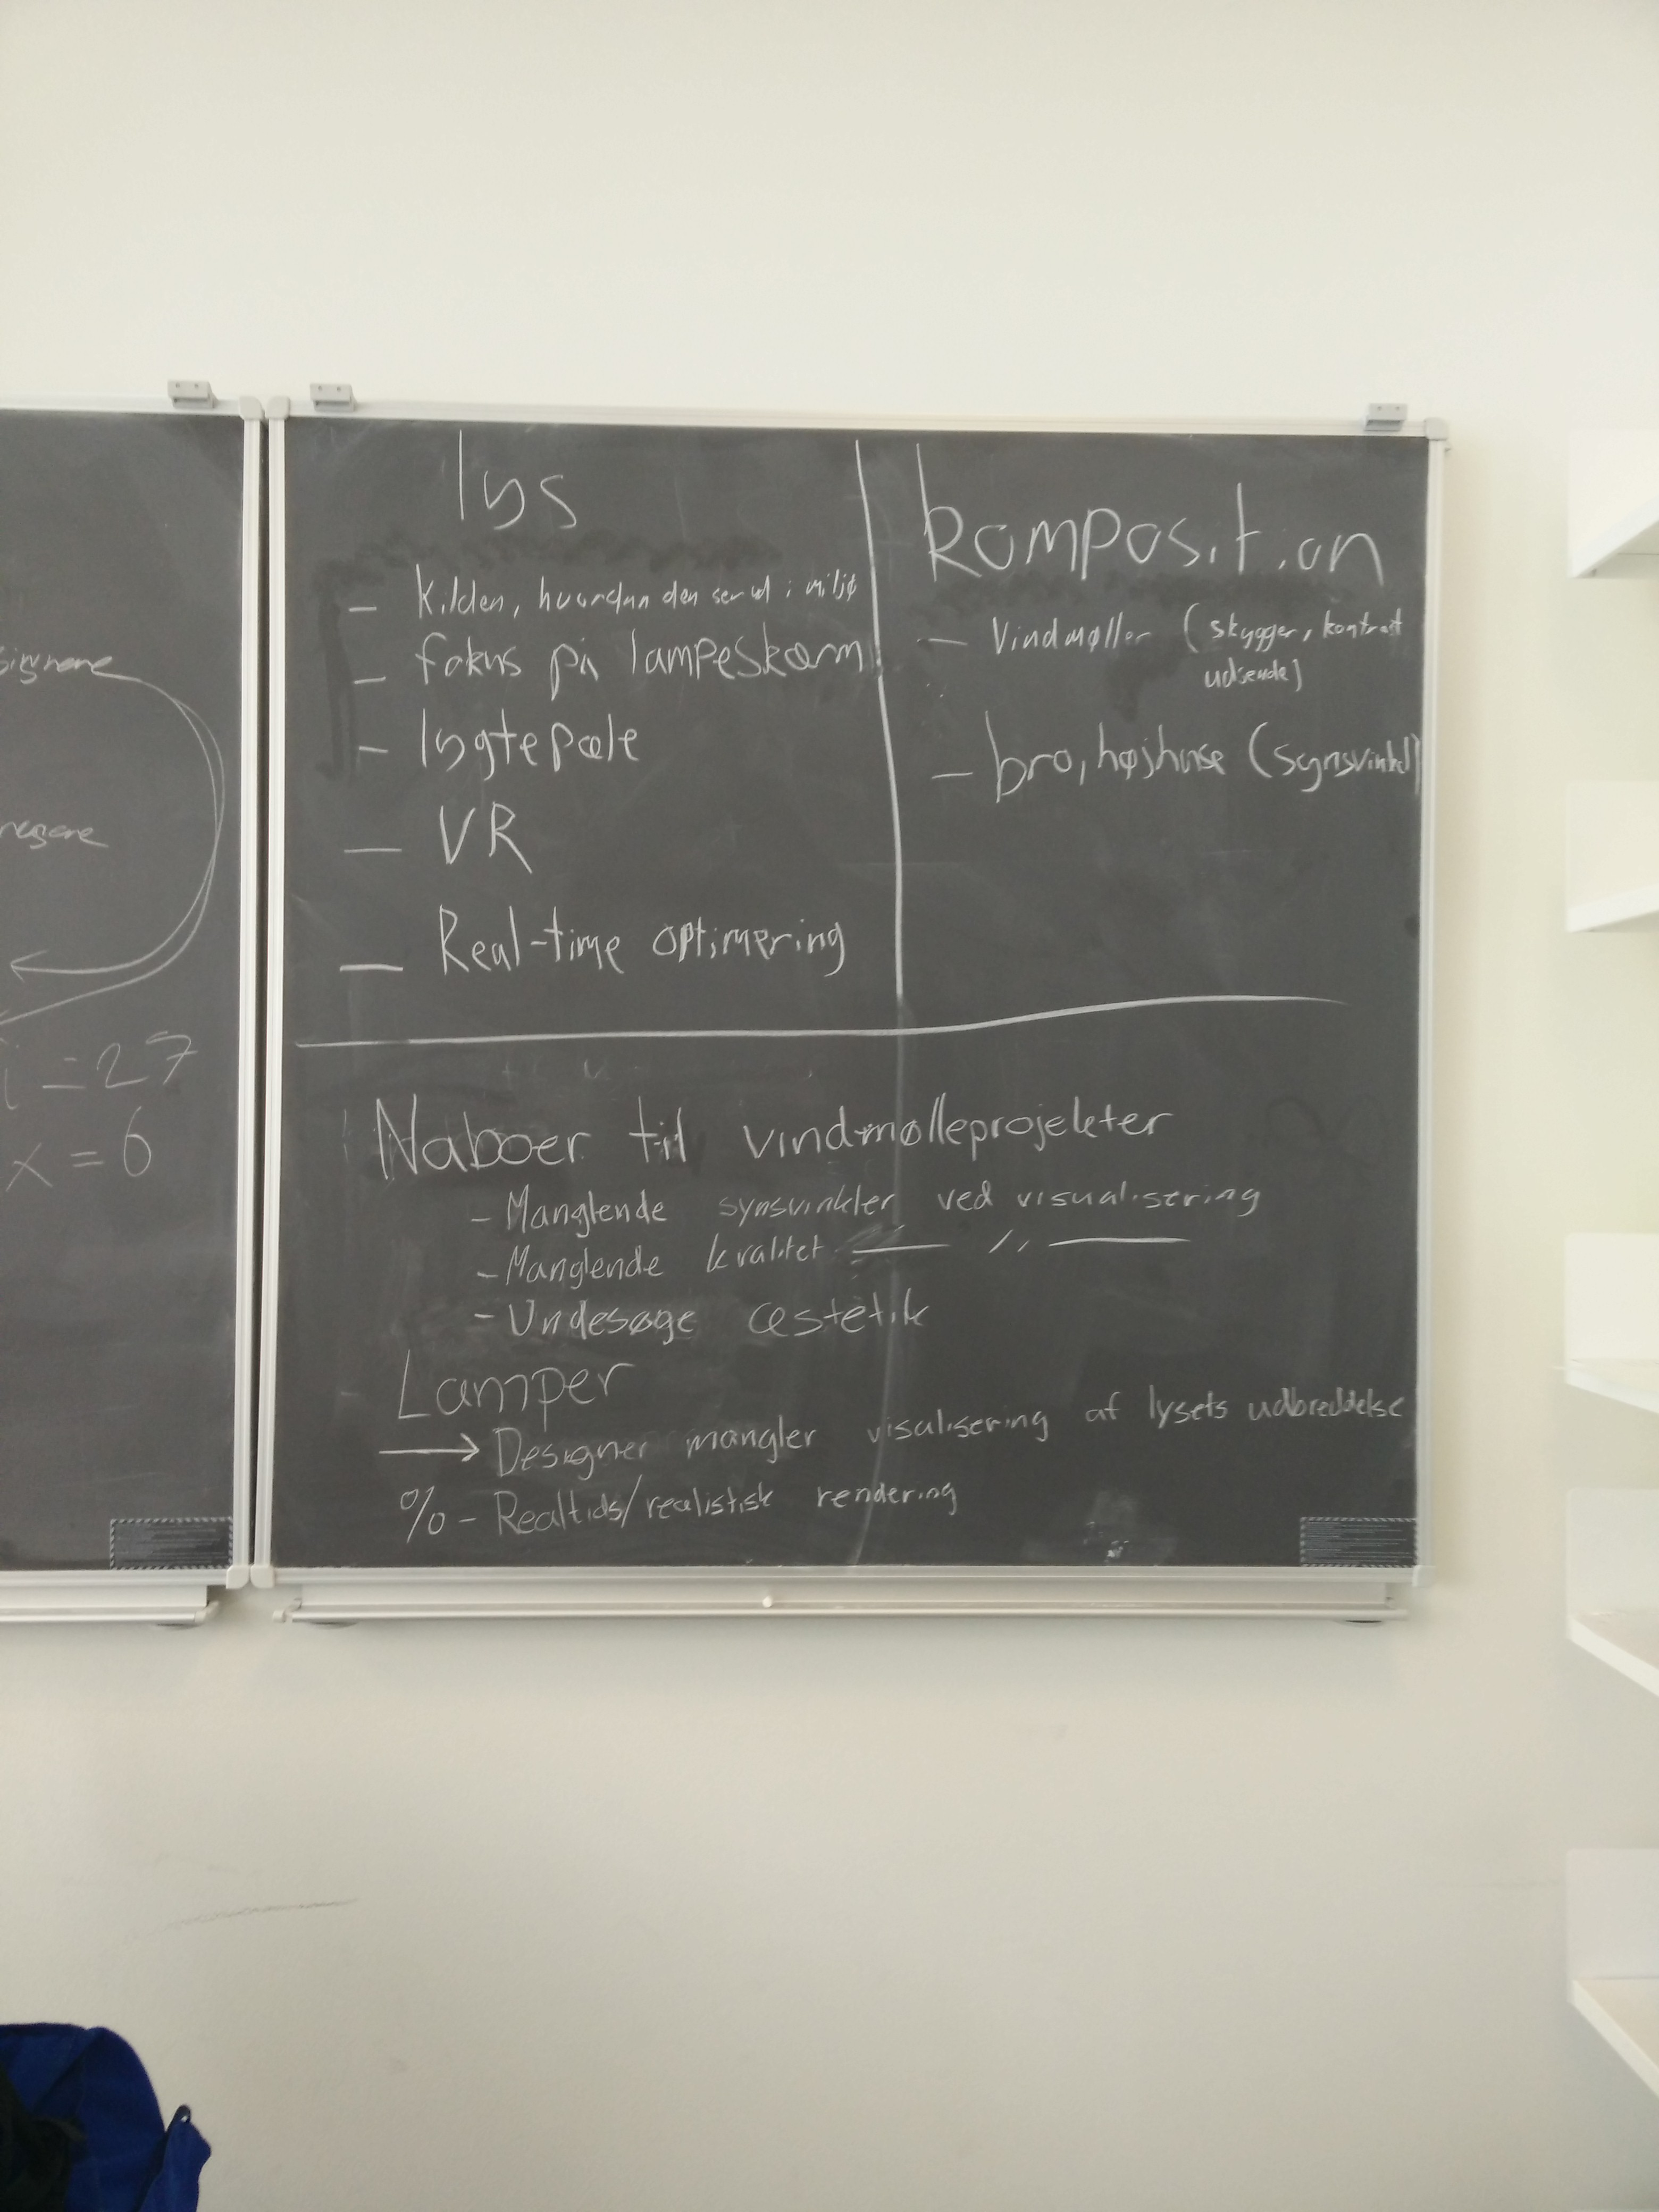
\includegraphics[width=10cm]{./../graphics/brainstorm_1}
\end{figure}

\subsection{Bilag D}

\subsubsection*{Trello}
\label{sec:trello}

\begin{figure}[H]
   \centering
   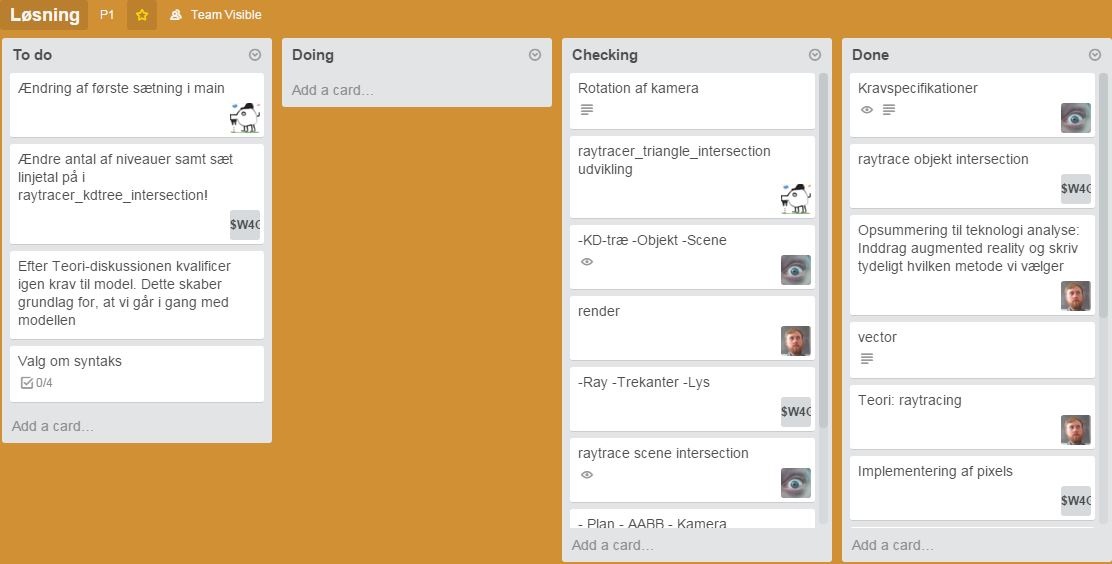
\includegraphics[width=10cm]{./../graphics/trello}
\end{figure}

\end{document}




